\setchapterpreamble[u]{\margintoc}
\chapter{Sensitivity of IceCube-Gen2 to measure flavour composition of Astrophysical Neutrinos}
\labch{gen2}
Siginificant portion of this thesis work was dedicated to assess IceCube Gen2's sensitivity to measure the flavour composition of the astrophysical neutrinos. The detector will be introduced in the following sections, along with the simulations and software framework used to produce the results. 

\section{IceCube Gen2} 
\label{sec:gen2-detector}
IceCube-Gen2 is a proposed next generation of neutrino detector, designed to observe the neutrino sky within a wide energy range, from TeV to EeV \sidecite{whitepaper}. Its sensitivity is expected to be at least five times better than IceCube, enabling the observation of individual sources. The instrument layout is designed to detect about ten times more neutrinos annually as compared to IceCube. This increased capability will facilitate in-depth studies of the distribution of neutrinos across the sky, energy spectrum, and flavour composition, as well as beyond-the-Standard-Mode.
\begin{figure}[h!]
	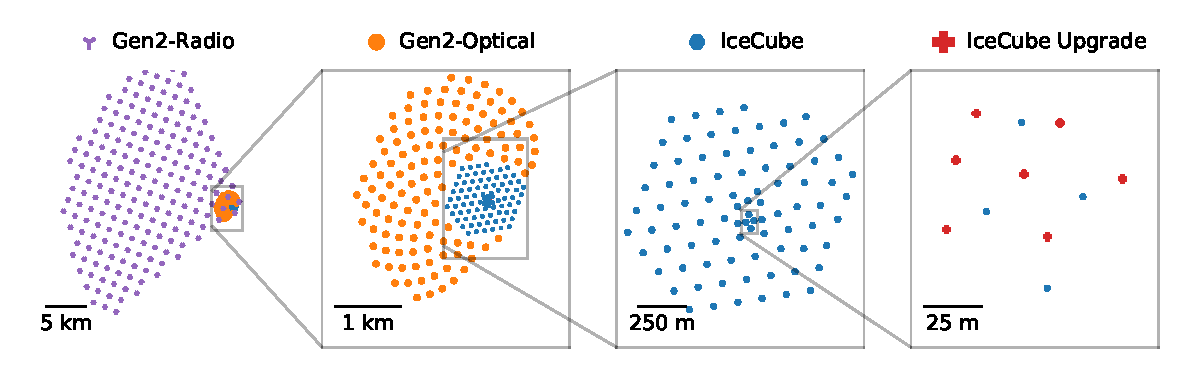
\includegraphics[scale=1.5]{./figures/gen2/decadal_survey_gen2-fan_radio_geometry.pdf}
	\caption[Layout of IceCube-Gen2 geometry]{Figure depicts the proposed IceCube-Gen2 Neutrino Observatory facility at the South Pole. It includes (from left to right) (i) a radio array with 200 stations, (ii) 120 new in-ice strings, spaced 240 m apart (shown as orange points), as an expansion of (iii) current optical array, (iv) 7 strings of IceCube upgrade, to be deployed soon within currrent in-ice DeepCore volume. Figure taken from \cite{whitepaper}}
	\labfig{gen2_all_geometry}
\end{figure}

\reffig{gen2_all_geometry} illustrates a top view of the IceCube-Gen2 facility, showcasing its various components using optimized technologies for the targeted energy ranges. 

\begin{description}
    \item \textbf{\emph{The IceCube Upgrade}} will start deployment this season (2024-2025 austral summer). Its goal is to lower the detection threshold for neutrinos to 1 GeV (In-line with its predecessor, \emph{DeepCore} in current IceCube)\sidecite{AYA}. This improvement will advance oscillation measurements, dark matter searches, and studies of physics beyond the Standard Model. The IceCube Upgrade project will also deploy 693 new multi-PMT detector modules on 7 new strings as shown in right-most panel of \reffig{gen2_all_geometry}, providing an opportunity to test the optical sensor technology for the IceCube-Gen2 observatory.

    \item \textbf{\emph{The Surface Array}} of IceCube-Gen2 is a setup of scintillator detector arrays on the surface of the South Pole, that measures the electromagnetic shower component and low-energy muons, while the optical array detects $\geq \mathrm{TeV}$ muons from the same air shower \sidecite{IceCubeCollaborationSchroeder2024_1000168735}. Planned to be used similarly as \emph{IceTop} of IceCube (see Section~\ref{sec:IC_detector}), the stations shall be placed on top of the additional \emph{in-ice} strings of optical array. It can also be used as \emph{surface veto} to reduce the background of atmospheric muons in samples of astrophysical neutrinos from the southern sky.

    \item \textbf{\emph{The Radio Array}} aims to discover and characterize the high-energy neutrino flux above 10 PeV. It detects nanosecond-scale radio emissions from ultra-high-energy particle showers using the Askaryan effect \sidecite{Askaryan,meyers_21}. This technique is sensitive to energies above a few PeV and complements the energy range of the optical array by capturing radio emissions from neutral and charged-current interactions, as well as energy losses of secondary leptons. The initial stations of the Radio Neutrino Observatory in Greenland, will serve as a R\&D tool for the Radio component of IceCube Gen2 \sidecite{rnog}.

    \item \textbf{\emph{The Optical Array}} The optical array will be expanded with the addition of 120 new strings to the existing IceCube strings. The strings will be arranged in what is referred to as "sunflower geometry," with an average horizontal spacing of 240 meters. The shape of the array and spacing between the strings will be determined through dedicated geometry optimization studies. Each string will contain 80 modules, resulting in a total of 9600 new modules. These modules will be placed between 1325 meters and 2575 meters below the surface, with a vertical spacing of 16 meters. This configuration will create an instrumented geometric volume of 7.9 cubic kilometers. The modules on the string are expected to collect nearly three times the number of photons gathered by an IceCube digital optical module (DOM) \sidecite{whitepaper}.
\end{description}

For the sensitivity study presented in this thesis, only the optical part of the proposed detector was simulated and used. 

\begin{figure}
	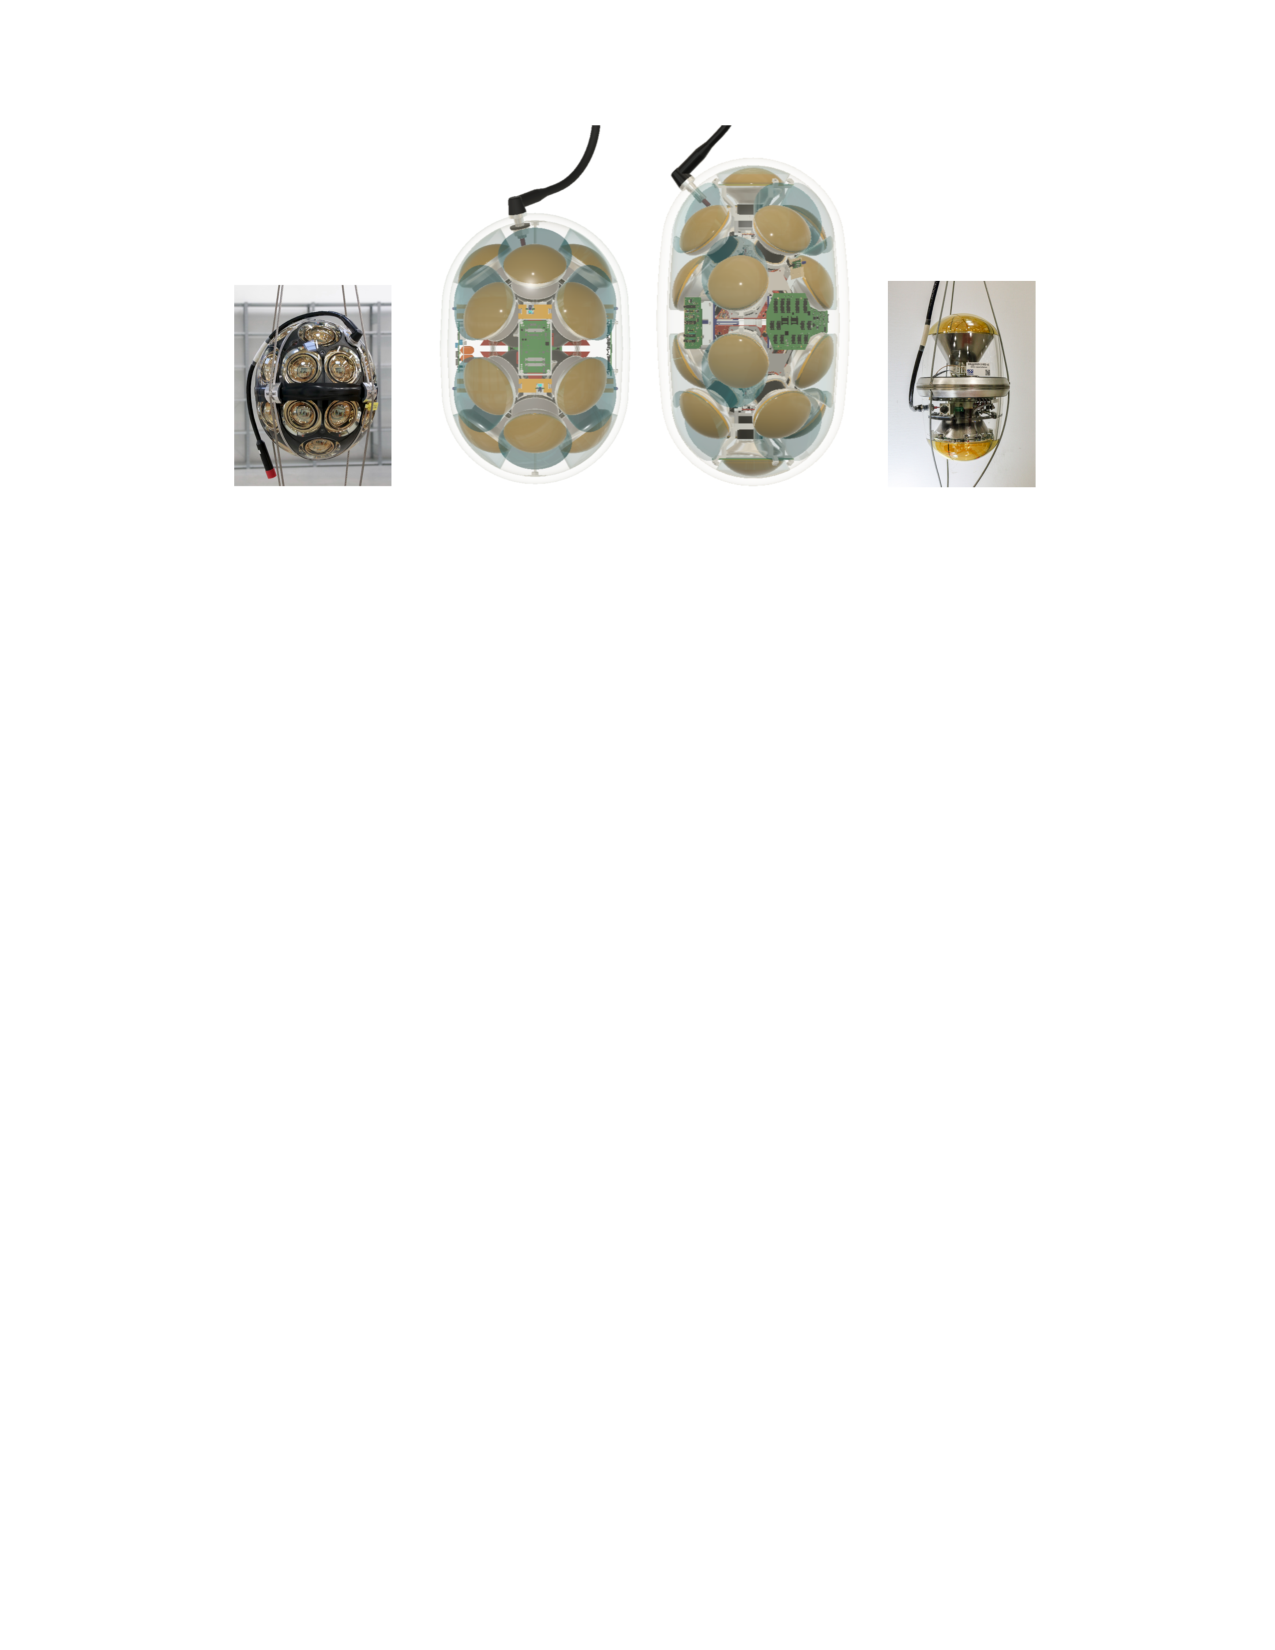
\includegraphics[scale=2.2]{./figures/gen2/Gen2_DOMs.pdf}
	\caption[Designs of candidate optical modules for IceCube-Gen2]{The designs of the IceCube-Gen2 optical sensors, DOM-16(second) and DOM-18 (third) with their base designs, to be used in the IceCube Upgrade sensors, are the mDOM on the left and D-Egg on the right \cite{Gen2_TDR}}
	\labfig{Gen2DOMs}
\end{figure}

\section{Simulation}
\label{sec:gen2-sim}
To perform this sensitivity study, dedicated simulations were carried out. The study aims not only to assess the sensitivity of IceCube-Gen2 for measuring the flavour composition of astrophysical neutrinos but also to evaluate its capabilities for detecting tau neutrino events, which is a crucial component as described in \refch{nu_samples}. The simulations were aligned with the mainline IceCube simulations (detailed in Section~\ref{sec:sim_ic}) to enable direct comparisons. However, necessary modifications were made to account for the new-generation optical sensors to be used in IceCube Gen2 and the sparser geometry. 

The following sections will describe the event samples created using these simulations to conduct the sensitivity analysis. First a brief overview of the \emph{simulated} sensor shall be given, where an isotropic sensor was created by assuming a spherical PMT, instead of a more realstic multi-PMT module, which requires considerable amount of time and resources to establish. The rest of the simulation chain remains identical to that explained in Section~\ref{sec:sim_ic} for mainline icecube simulations,
\begin{kaobox}
    particle generation $\rightarrow$ propgation of secondaries $\rightarrow$ photon propagation $\rightarrow$ Detector Simulation 
\end{kaobox}
Once the simulation is available, the selection cuts are applied to select only high energy events that starst within the detector volume, to mimic the so-called High Enegy Starting Event (HESE) described in Section~\ref{sec:HESE}. A classification of all HESE-like\sidenote{The selection is reffered as HESE-like and not exactly HESE as the original selection is sensitive to the detector geometry where outer layer DOMs are used as an active veto as described in Section~\ref{sec:HESE}. For this sensitivity
 study, an approximation was made by matching the effetive area of sample derived using IceCube-only strings.} events is then performed using a similar particle identifier described in Section~\ref{sec:PID} to classify these events in three morphologies, \textbf{Single Cascade,Double Cascades and Tracks}. 
\subsection{Isotropic Sensor}
\label{sec:isopdom}
The choice of optical sensors to be used in the IceCube-Gen2 project depends strongly on how well the reference optical sensors to be deployed in the IceCube upgrade perform.\sidecite{Gen2_TDR}. The designs have been carefully optimized to balance cost-effectiveness, logistical efficiency, and enhanced performance. \reffig{Gen2DOMs} shows both the 16 and 18 PMT modules, which are being considered to use in IceCube Gen2, along with \textbf{mDOM} (\emph{multi PMT Digital Optical Module}) \sidecite{mDOM_2017,mDOM_2019} and \textbf{D-Egg} (\emph{Dual optical sensors in an Ellipsoid Glass for Gen2}) \sidecite{D-Egg_MainPaper} that are to be deployed in ice for IceCube Upgrade.

\marginnote{\begin{kaobox}[title=pDOM]
    pDOM stands for PINGU Digital Optical Module. It was first coined for an R\&D upgrade of IceCube DeepCore called \textbf{PINGU} (The Precision IceCube Next Generation Upgrade) \cite{PINGU}.
\end{kaobox}}

The maturity of the design, along with extensive in-situ testing using a large number of sensors for the IceCube Upgrade, leads us to consider the mDOM-type sensor as the baseline for evaluating the IceCube Gen2 detector's capabilities in identifying Tau neutrino-induced Double Cascade events. Unlike IceCube’s single large 10" PMT, the mDOM consists of 24 smaller 3" PMTs. The key advantages of the mDOM over pDOM \sidecite{PINGU} are its 2.2 times higher effective photocathode area, omnidirectional sensitivity, and the directional information obtained from the individual “pixels” (the 24 PMTs). Due to the large number of PMTs and their strategic placement within the module sphere, this module offers nearly isotropic angular acceptance, unlike IceCube DOMs with only one downward-facing PMT. 

The effective area of the optical modules is the equivalent physical cross-section that would detect all the incident photons from a plane perpendicular to a given direction. As illustrated in \reffig{EffectiveArea_mDOM} (Left plot), the mDOM has a nearly constant effective area for collecting photons from all directions, unlike the Gen1 DOMs (pDOMs) which have a downward-facing PMT. As a result, the effective area for pDOMs increases as the arrival direction shifts from 180 degrees ("down-going" in the IceCube coordinate system) to 0 degrees ("up-going" in the IceCube coordinate system).

\begin{figure}
    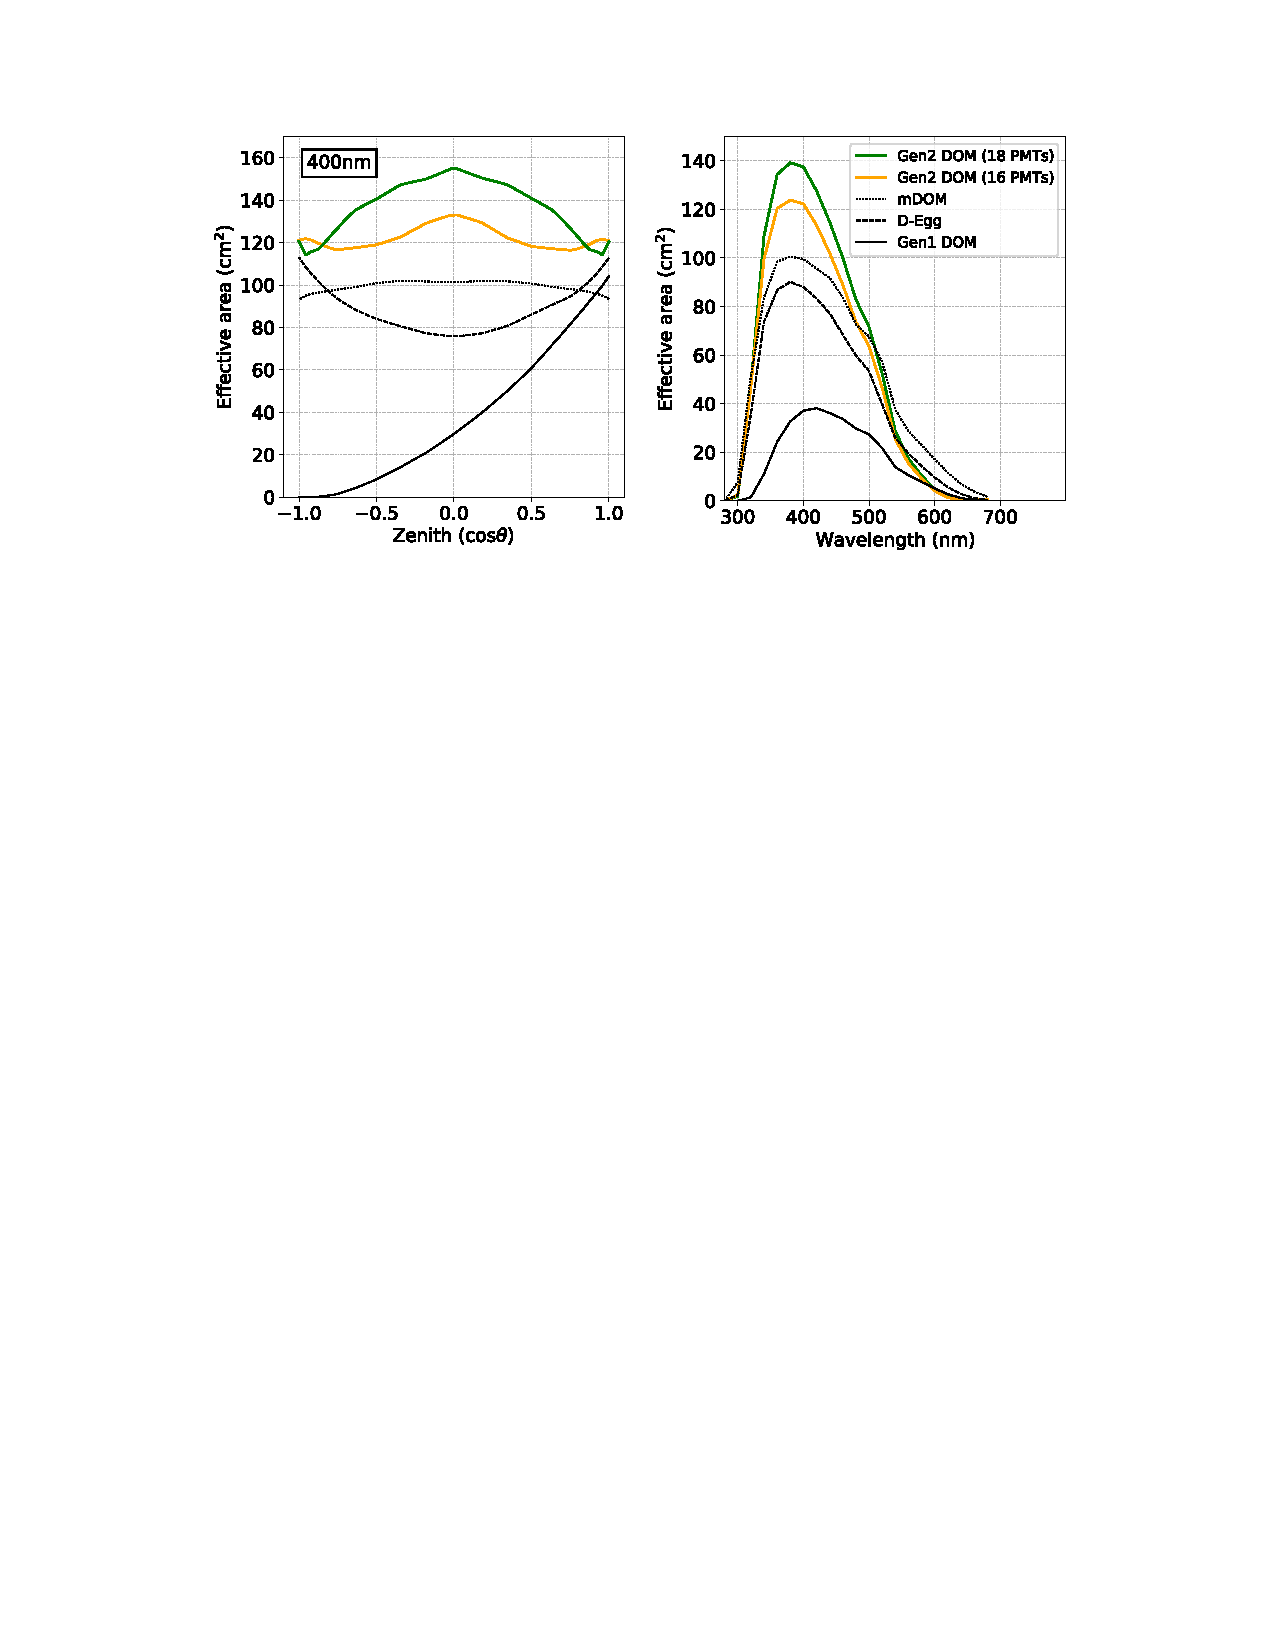
\includegraphics{./figures/gen2/EffectiveAreaCurve_TDR.pdf}
    \caption[DOM effective area comparisons of Multi-PMT modules with a current single PMT DOM of IceCube]{The effective area is compared for IceCube-Gen2 DOM candidates, 16, and 18 PMT models, in relation to IceCube-Gen1 DOM (pDOM), D-Egg, and mDOM, as functions of zenith angle (left) and wavelength averaged over solid angle (right). Figure taken from \cite{Gen2_TDR}} 
    \labfig{EffectiveArea_mDOM}
\end{figure}

However, current simulation methods used in IceCube (see Section~\ref{sec:mc_sim}) do not yet provide a detailed simulation of a multi-PMT module, so a simulated sensor called \emph{iso-pDOM} (isotropic-pDOM) was developed \sidecite{Anastasiia_Thesis}. This sensor can be thought of as a 'spherical PMT' encased in a glass vessel similar to an IceCube DOM but with 2.2 times higher quantum efficiency, capable of capturing photons arriving from all the directions (see \reffig{isoPDOM_schematic}). The sphere was simulated by assuming an upward-facing PMT along with a downward one and combining the results while maintaining the same area under the curves at all wavelengths. The resultant iso-pDOM has an effective area very similar to that of an mDOM.

\begin{marginfigure}
    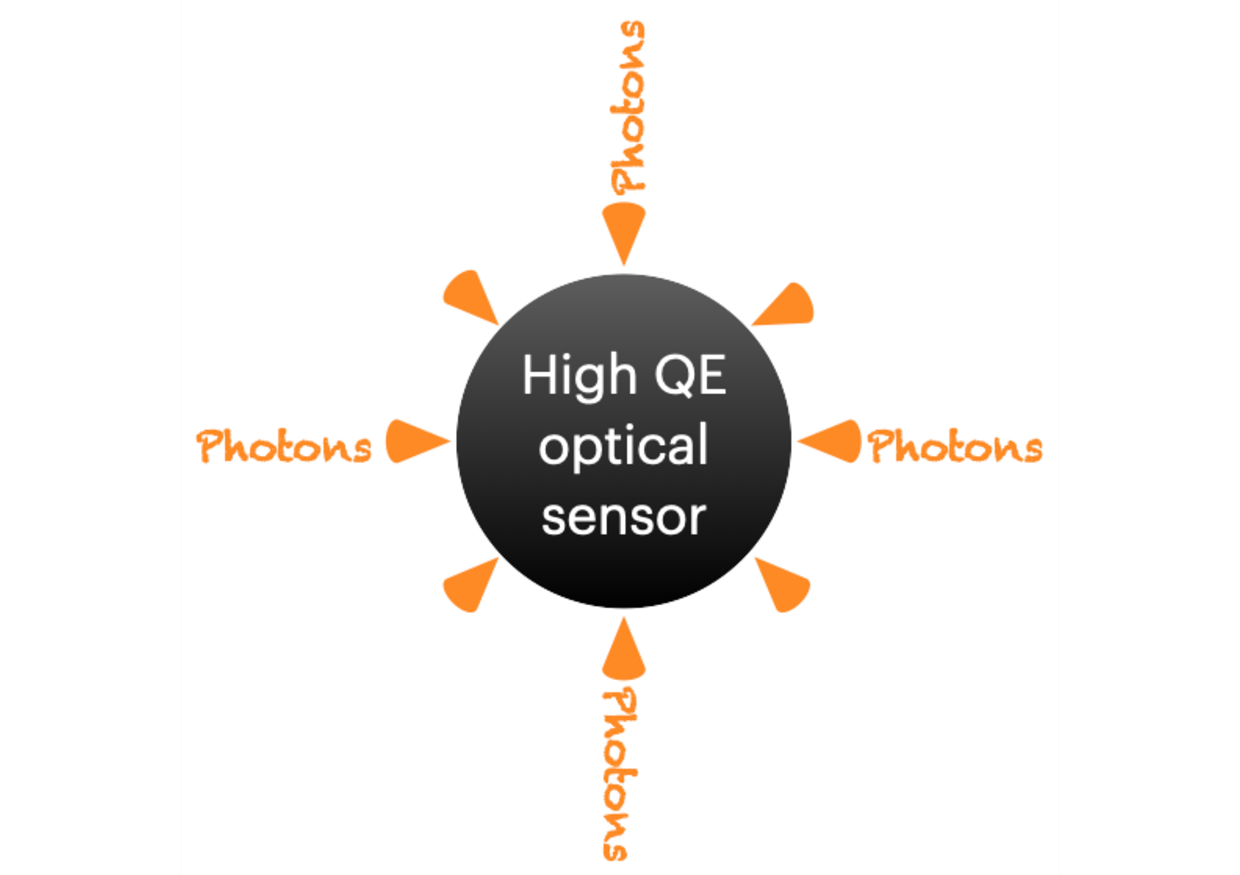
\includegraphics{./figures/gen2/iso-pDOM.pdf}
    \caption[Schematic of an isoPDOM]{Conceptual representation of Simulated sensor with isotropic angular acceptance (iso-pDOM)}
    \labfig{isoPDOM_schematic}
\end{marginfigure}

\begin{figure}
    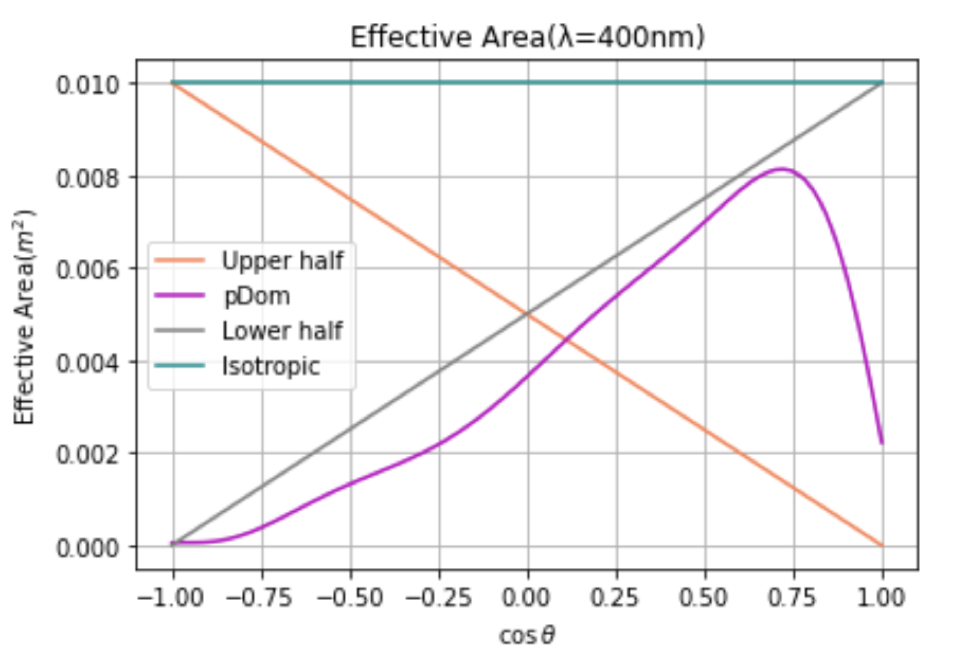
\includegraphics{./figures/gen2/isopDOM_eff_area.png}
    \caption[Effective area of isoPDOM]{Results of simulating a sensor that \emph{mimics} the behaviour of a typical mDOM. The blue line shows changed effective area of the so-called \emph{isopDOM}, achieved by combining acceptance curves of pDOMs having a PMT in "upper" (orange) and "lower" (grey) halves of the DOM respectively}
    \labfig{isoPDOM_effarea}
\end{figure}


\subsection{Event Selection}
\label{sec:gen2_eventsample}

Monte Carlo events were produced using isoPDOM for all three flavours of primary neutrinos with energies ranging from 100 TeV to 50 PeV. The simulation chain is identical to that described in Section~\ref{sec:mc_sim}. It is important to note that since the IceCube in-ice array is inherently part of the proposed Gen2 detector, all simulated events still include information (collected charge) collected by IceCube DOMs from the IC86\sidenote{IC86 stands for the current IceCube detcetor volume, made up of 86 strings containing Digital Optical Modules (DOM).} configuration. Additionally, during the Detector Simulation stage of the simulation chain (see Section~\ref{sec:mc_sim}), where PMT responses, noise, etc., are added, responses are incorporated separately for IceCube DOMs and isoPDOMs. If an event passes all the basic triggers, two separate triggers are stored depending on the event location: IC86 and ICGen2. By default, ICGen2 has a combined response of both detector configurations, while IC86 only contains current IceCube volume events. This feature is crucial as it facilitates direct comparison of events produced with IceCube simulations for IceCube-only analyses.

A fundamental aspect of flavour measurement studies is the ability to identify the flavour of the neutrino involved in an interaction. This identification is possible due to the distinct by-products produced by different neutrino interactions, which result in unique light deposition patterns, or "morphologies" as described in Section~\ref{sec:morphologies}. These patterns, illustrated in \reffig{topologies}, allow us to reconstruct the events by analyzing the pattern of photon detections in the detector. By doing so, the flavour of the original interacting neutrino can be determined.

To utilize the same particle identifier used in the analysis preseneted in \refch{analysis} for this sensitivity study, a dedicated event selection process for high-energy starting events (HESE) \sidecite{HESE7_sample} was implemented. However, since the outer-layer detector veto is specific to the detector geometry and the characteristics of the DOM pulses—which is still under development for the IceCube-Gen2 simulation chain-starting events were selected by examining the interaction vertex of the primary neutrino. This interaction vertex was further refined by considering the deposited charge (measured in single photoelectrons) and calculating the charge-weighted mean positions. This charge information is crucial for applying a HESE-like charge cut. Unlike the 6000 photoelectrons threshold used previously, the threshold for this analysis was set at 2000 photoelectrons. The lower threshold is due to the higher quantum efficiency and isotropic sensitivity of the new sensors, which enhance the detection capability for high-energy events. All the approximations made were in parallel checked for IC86 configuration to reproduce Monte Carlo PDFs within statstical erros to the ones presented in analysis chapter.

Moreover, to appropriately weight the simulated events and account for the probability of an atmospheric neutrino being rejected by an accompanying muon triggering the veto, a dedicated calculation similar to the one used in the HESE-7.5 analysis \sidecite{HESE7_sample} was used. Additionally, the reconstructed energy cut, initially set at 60 TeV, was adjusted to 100 TeV. This adjustment was based on the signal-to-background probability density functions (see \reffig{DC_PDFs}) to ensure a similar signal-to-background ratio (2:1) as achieved in the HESE-7.5 analysis \sidecite{Juliana_paper} and the HESE-12 analysis, presented in \refch{analysis} and \refch{HESE12}. A peculiar observation while looking at Monte Carlo PDFs shown in \reffig{DC_PDFs} compared to those shown in \reffig{LvsE_signalbkg} can be seen due to limited number of produced Monte Carlo for this study. Although, even with low stastics, more population along the LvsE diagonal is clearly visible on the left panel showing signal Double Cascade events. 

After applying all the necessary filters, the final sample includes starting events with a reconstructed deposit energy of 100 TeV or more and a charge exceeding 2000 PE. These events originate from interactions of all six types of neutrinos (particle and antiparticle versions of 3 flavours) beginning within the simulated IceCube-Gen2 fiducial volume. They are divided into three categories: Tracks, Single Cascades, and Double Cascades.

\begin{figure*}[h]
    \begin{subfigure}[h]{0.7\textwidth}
        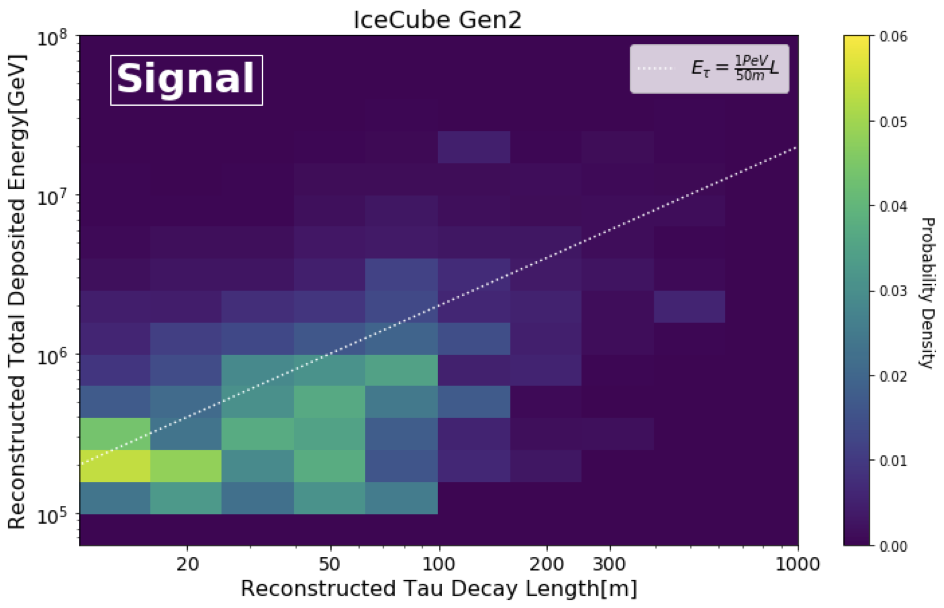
\includegraphics{./figures/gen2/Signal_PDF.png}
    \end{subfigure}
    \hfill
    \begin{subfigure}[h]{0.7\textwidth}
        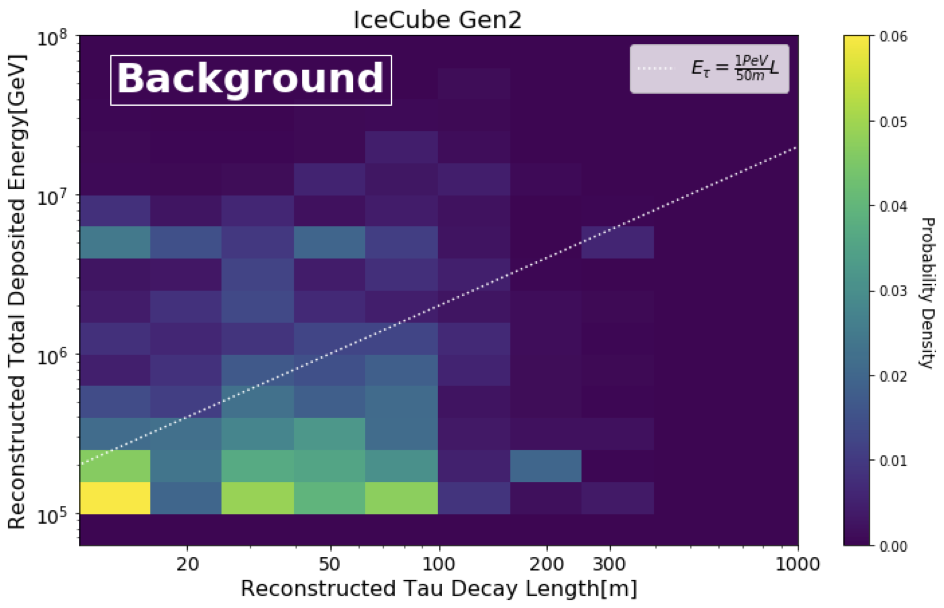
\includegraphics{./figures/gen2/Bkg_PDF.png}
       
    \end{subfigure}
    \caption[2D Monte Carlo PDFs of reconstruct energy and length for double cascade events in IceCube-Gen2]{Two dimensional Monte Carlo templates, constructed using reconstructed total energy ($E_{\text{Tot}}$) and double cascade length ($L_{\text{dc}}$) for events classified as \textbf{double cascades}. The signal (left), representing $\nu_\tau$-induced double cascades, shows a clear correlation between $L_{\text{dc}}$ and $E_{\text{tot}}$. In contrast, the background (right), consisting of $\nu_\mu$ and $\nu_e$ events, lacks this correlation and clusters at low $L_{\text{dc}}$.}
    \labfig{DC_PDFs}
    
\end{figure*}


\section{Analysis tool : \texttt{toise}}
\label{sec:toise}
Understanding and enhancing the sensitivity of the detector can result in more precise and dependable performance, thus improving the scientific impact of the experiment. The main goal of the sensitivity studies carried out in this work is to optimize the design of the detector in order to be capable of reconstructing tau neutrino events using existing methods, but with a larger detection volume and new generation optical sensors. Additionally, one can also assess the sensitivity of the detector by combining both radio and optical arrays of the proposed detector to investigate flavour measurements in the energy ranges from TeV to EeV \sidecite{Coleman}.

It's impractical to run comprehensive simulations for evolving detector designs due to the large amount of computing power required. The \texttt{toise} \sidecite{toise} framework was created to estimate sensitivity using a simplified model of the detector response based on targeted Monte Carlo (MC) simulations. This allows for efficient comparisons of different detector designs without repeating the entire simulation process. \texttt{toise} was used for a sensitivity study presented in the next section. This section will provide a brief overview of its workflow. In order to distinguish the influence of design choices on detector performance from the intrinsic restrictions imposed by neutrino interaction physics, the event rate calculation in this framework is conducted through two distinct stages: Neutrino Physics and Detection.

In the Physics stage, the neutrino fluxes at the Earth's surface are converted to the detector's area or volume. This involves using a transfer tensor to model the conversion between the initial neutrino flavour states and the observable final states (muons, hadrons, etc.). In addition, various aspects of neutrino interactions, including neutrino-nucleon cross-sections and different interaction types (neutral current or charged current) are also taken into account. The transfer tensor is subsequently combined with the final-state effective area to establish a neutrino effective area. The effective area \( A_{\text{eff}}(E, \theta) \) of the detector is calculated by multiplying the geometric area \( A_{\text{geo}}(\theta) \) with an energy and zenith-dependent efficiency \( \eta(E, \theta) \):

\begin{equation}
    A_{\text{eff}}(E, \theta) = A_{\text{geo}}(\theta) \times \eta(E, \theta)
\end{equation}

For the optical array of the proposed IceCube-Gen2, the geometric area is approximately calculated by placing a convex hull around the instrument's geometric boundary. \textbf{\emph{The selection efficiency}} \( \eta(E, \theta) \) characterizes the detector's triggering efficiency and the probability of an event passing a set of analysis criteria. It is defined as \emph{the ratio of events passing these cuts to the number of events generated}. Depending on the type of sensitivity study being performed—such as expected limits, discovery potential, or flavour measurement—additional parameterizations like energy and angular resolutions and classification efficiency are used. For flavour measurement, \textbf{\emph{the classification efficiency}} generates an event classification smearing matrix (\reffig{classeff}) and is defined as \emph{the fraction of morphology per energy bin for a given neutrino flavour}.

When estimating sensitivities, it is essential to account for backgrounds that may mimic the signal. The framework handles backgrounds by either adding their contributions to the event rate or ignoring regions where they are expected to contribute. For all detectors and science cases, atmospheric neutrino flux is added as a background using the same effective area as for astrophysical neutrinos. Optionally, atmospheric neutrino flux in the downward-going region can be reduced to account for vetoing by accompanying muons from the same air shower. This is done in a similar way to the one described in Section~\ref{sec:selfveto}.

\section{Result of Flavour Sensitivity Measurements}
\label{sec:gen2-results}
Using the HESE-like sample, described in Section~\ref{sec:gen2_eventsample}, a detector response tensor is generated using \texttt{toise}. Selection efficiency, detailed in Section~\ref{sec:toise}, is a key factor in generating the detector's neutrino effective area. This efficiency is determined using \reffig{selecteff}, which shows the true deposited energy at which the analysis starts to select events. The plot illustrates the ratio of events passing all selection cuts in Section~\ref{sec:gen2_eventsample} to all simulated neutrinos reaching the fiducial volume, per energy bin. The curve is fitted, and the resultant plot shows that neutrinos are selected starting from approximately 200 TeV. This value is used as the selection threshold for events beginning or contained in the fiducial volume.

\begin{figure}[h!]
    \centering
      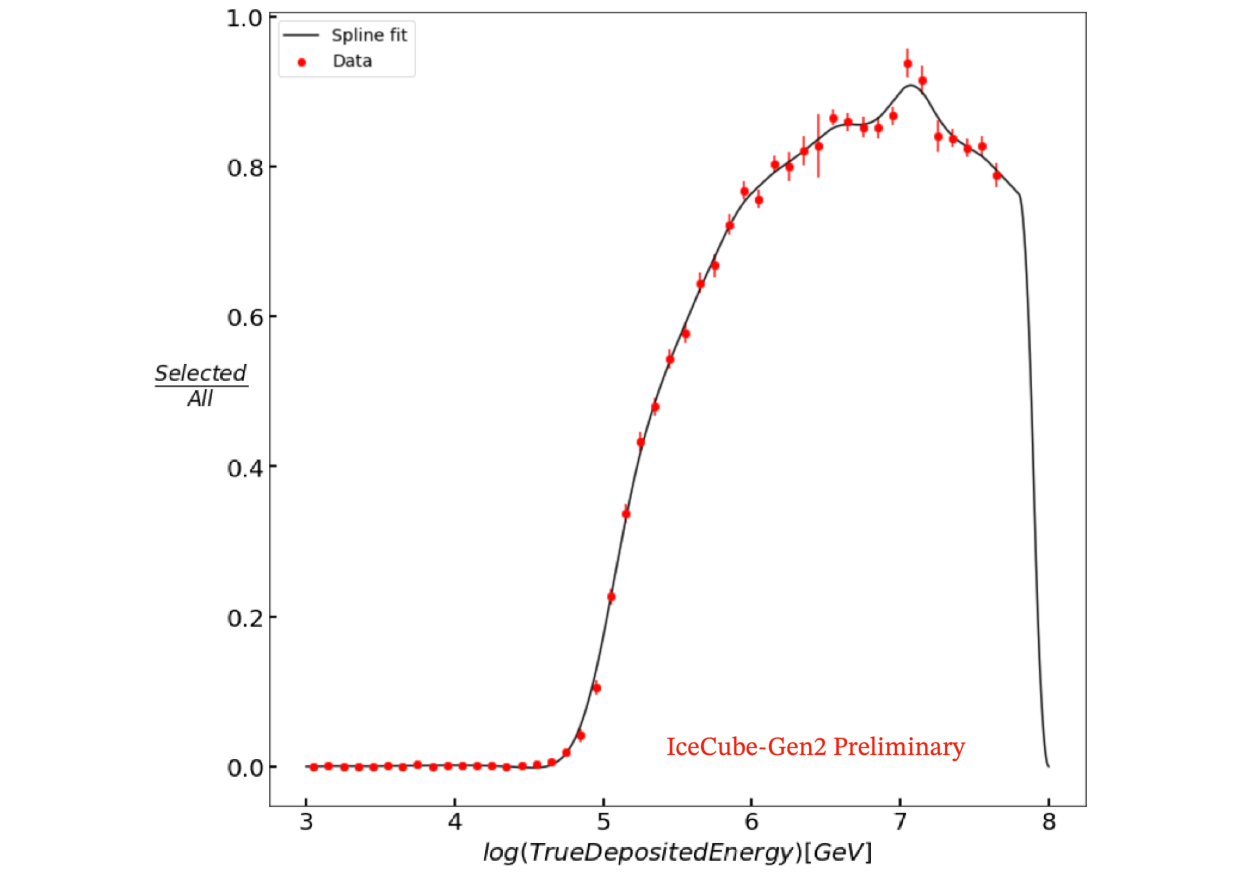
\includegraphics{./figures/gen2/SelectionEff.pdf}
      \caption[Selection Efficiency of HESE-like selection in IceCube-Gen2]{Selection Efficiency : Ratio of neutrinos that got classified into a morphology to all the neutrinos that interacted in active volume. Data here refers to monte-carlo events per energy bin.}
  \labfig{selecteff}
  \end{figure}


A specific parameterized tensor is used to determine the efficiency of particle identification during flavour measurements. \reffig{classeff} shows how well the reconstruction process can identify different types of particles based on their morphologies. In an ideal scenario, events involving charged current interactions with electron neutrinos ($\nu_e$) are classified as single cascades, those involving muon neutrinos ($\nu_{\mu}$) as tracks, and those involving tau neutrinos ($\nu_{\tau}$) as double cascades. The diagonal elements of the plot show how accurate the classifier is, while the off-diagonal elements indicate the fractions of misidentified flavours. The plot shows that as the true deposited energy increases, the number of double cascade events (from $\nu_{\tau}$ interactions) initially plateaus and then decreases. This occurs because at higher energies, the individual energy depositions are further apart (due to correlation of $\mathrm{L}_{\mathrm{dc}}$ and $\mathrm{E}_{\mathrm{tot}}$), making it easier for the reconstruction process to distinguish them. However, at even higher energies, one of the cascades may be partially or completely outside the detector, causing these events to be misclassified as single cascades due to strict containment criteria, as described in Section~\ref{sec:PID}. For single cascades involving $\nu_e$, the efficiency decreases at high energies because some DOMs may become saturated, and their data is excluded from the analysis. In contrast, the efficiency for starting tracks remains relatively consistent across the entire energy range.


\begin{figure}[h!]

    \centering
    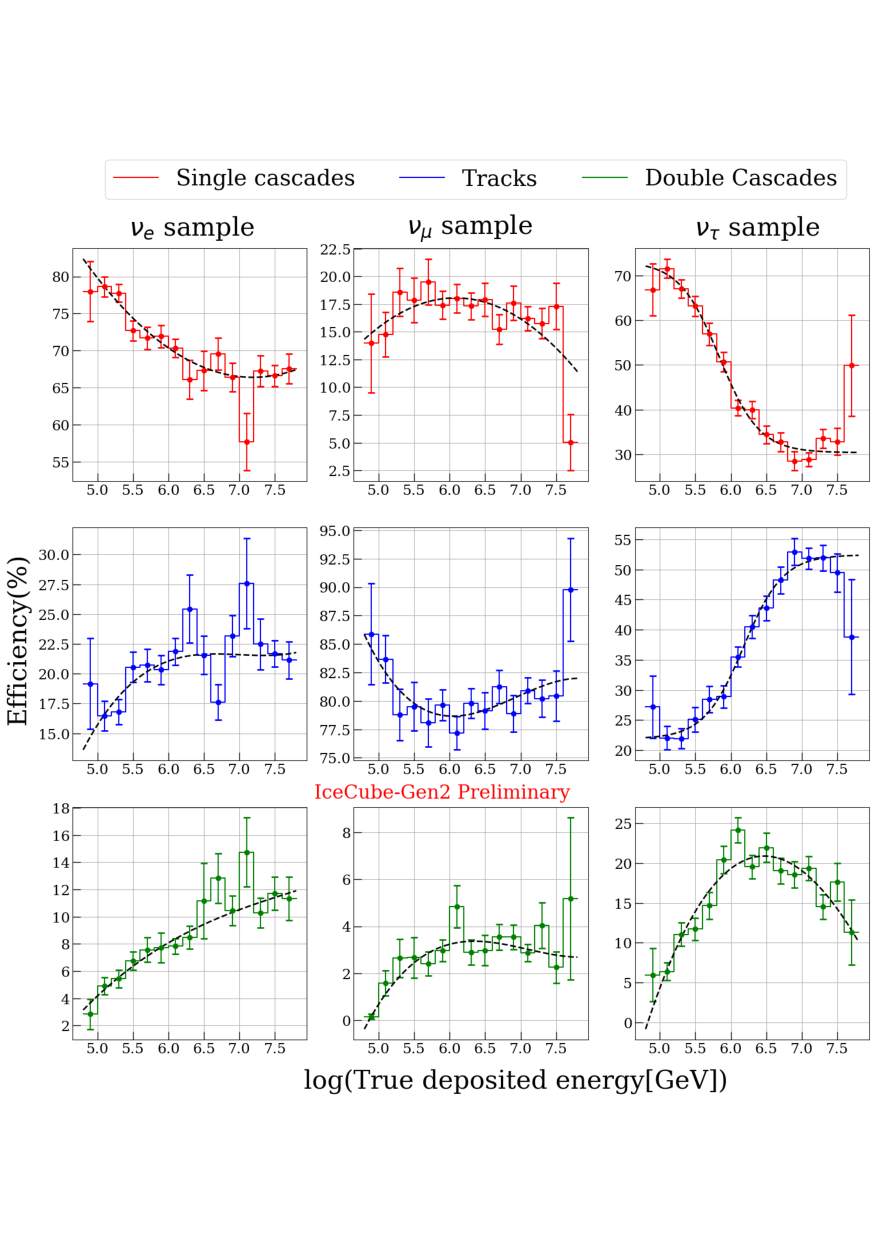
\includegraphics{./figures/gen2/ClassificationEff_small_watermark.pdf}
    \caption[Classification efficiency of a ternary particle identifier for IceCube-Gen2]{Classification Efficiency: Three subplot columns are true neutrino flavours, where each energy bin (true Monte Carlo energy) contains the fraction of topologies, summing to 100\%. Diagonal plots show the flavour identification efficiency of the classifier, whereas off-diagonal plots show misidentification fractions.
    }
    \labfig{classeff}
\end{figure}

Lastly, a significant advantage of \texttt{toise} is its ability to combine different event selections and detector types. The starting event sample from this detailed study can be combined with the efficiencies of other samples, such as through going tracks sample. In \texttt{toise}, these efficiencies are included by limits derived from IceCube analysis \sidecite[-2cm]{diffusenumu} to calculate angular resolutions, PSF, etc. The flavour measurement presented here demonstrates the sensitivity of IceCube Gen2 by combining starting events with through-going muons, a method already realized in IceCube \sidecite[-2cm]{Neha_ICRC_IC}.

\reffig{Gen2_flavourtriangle} shows the projected flavour measurement sensitivity of IceCube-Gen2 with 10 years of data \sidecite{Neha_ICRC_Gen2}. It is derived by using an asimov dataset \sidecite{asimov} assumes equal partition of all flavours, with a diffuse neutrino spectrum following a single power-law with an index of 2.5 and a per-flavour normalization of 2.3 \sidecite{lars_globalfit}. The confidence intervals are derived by assuming wilks' theorem \sidecite{Wilks_thm}, as for analysis presented in \refch{HESE12}. The figure also illustrates the sensitivity change if a dedicated $\nu_{\tau}$ identifier is not included in the starting event sample, resulting in the sample containing only single cascades and tracks, making it impossible to resolve the $\nu_e$ and $\nu_{\tau}$ fraction degeneracy. The systematic variations arising due to detector are neglected. 

\begin{figure}[h!]
    
    \caption[Sensitivity of IceCube-Gen2 to measure flavour composition of Astrophysical neutrino with 10 years of its lifetime]{Projected sensitivity of IceCube-Gen2 to measure flavour composition of Astrophysical neutrino with 10 years of its lifetime. The maroon line shows sensitivity using the ternary classification scheme and light salmon shade shows sensitivity \textbf{without} a dedicated $\nu_{\tau}$ identifier. The unresolved degeneracy along $\nu_e$/$\nu_{\tau}$ axis is notable due to lack of double cascade classifier. The solid (dashed) lines depict the corresponding 68\% (99\%) constraints, derived assuming Wilks' theorem.}
    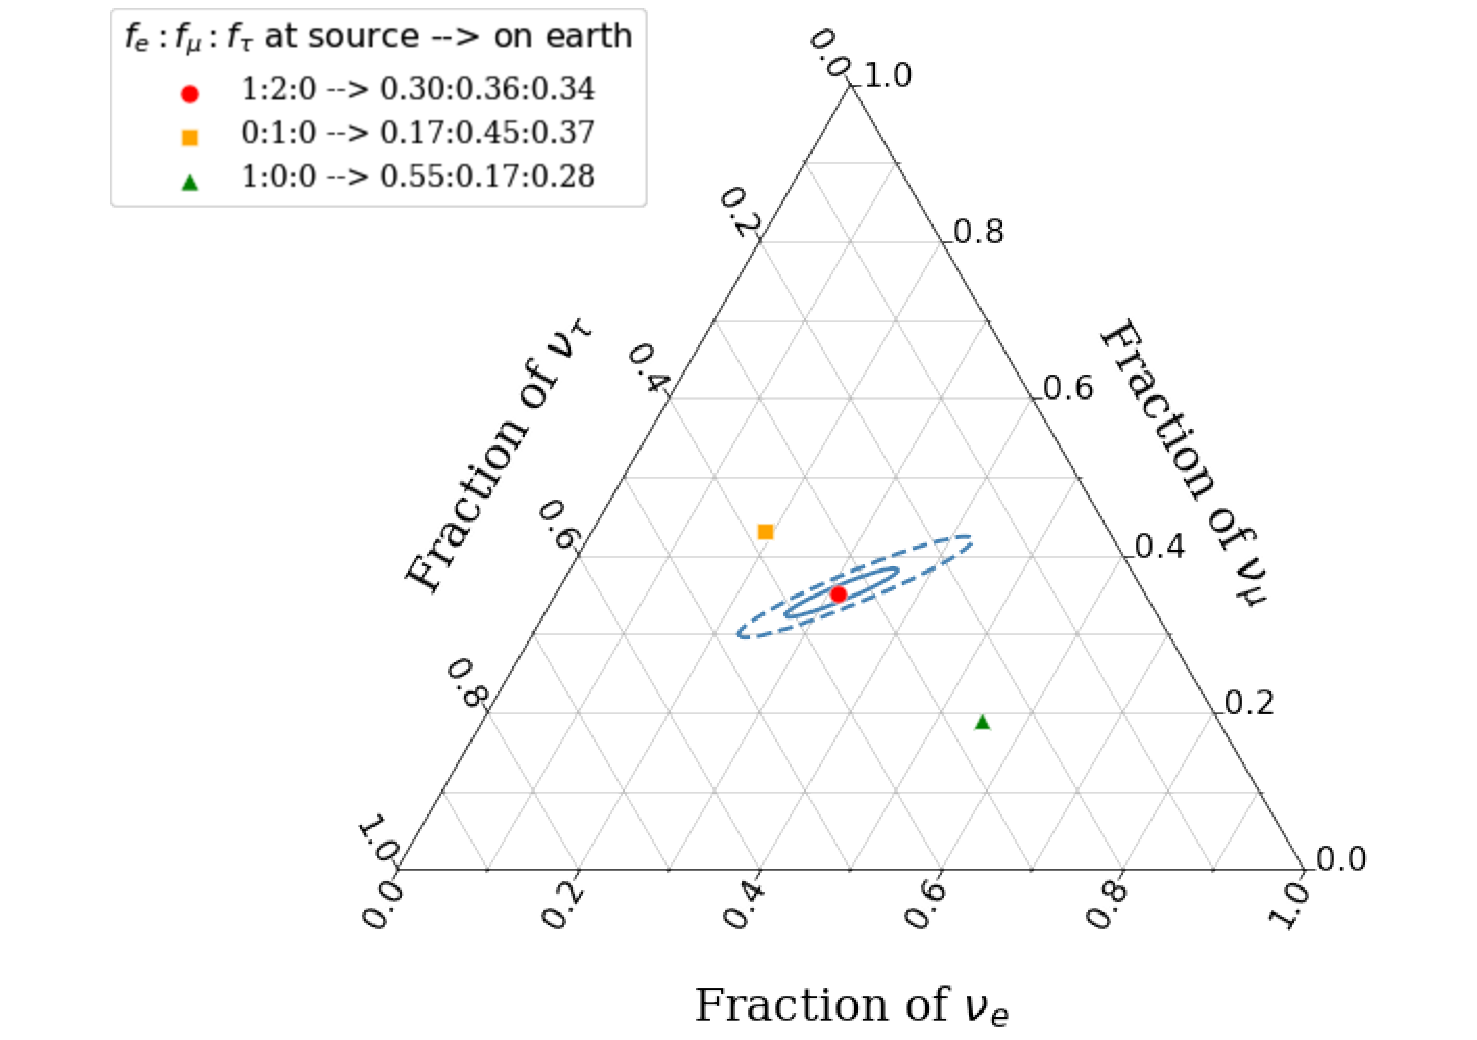
\includegraphics{./figures/gen2/Gen2-10Years.pdf}
    
    \labfig{Gen2_flavourtriangle}
\end{figure}

The sensitivity shown in \reffig{Gen2_flavourtriangle} and applies to the entire diffuse neutrino spectrum. With this study, flavour measurement for a given 'slice' of energy was also done to characterize its energy dependence. As described in Section~\ref{sec:astro_nu}, diffuse neutrino spectrum consists of neutrinos originating from various high-energy sources in all directions. Depending on the environments of the acceleration sites (magnetic fields, accretion disks, dust, etc.), the production ratios of neutrinos at the sites may differ \sidecite{cite166}. The most commonly assumed model, is the pion decay scenario (see Section~\ref{sec:flavour_theory}). At higher energies, however, due to synchrotron cooling of secondary muons produced in pion decay (see Equation~\ref{eq:pipm_decay}) the flavour production at sources changes to a ratio of ($\nu_e:\nu_{\mu}:\nu_{\tau}$) from 1:2:0 to 0:1:0 \sidecite{walter_muondamped}. If such sources begins to dominate the overall flux at high energies, a transition in measured neutrino flavour fluxes can be observed \sidecite{muon_damp}. \reffig{gen2_muondamped} shows IceCube-Gen2's sensitivity to detecting such a flavour transition. The assumed "critical energy" for this mechanism for the study is 2 PeV. This transition is detectable with IceCube-Gen2 due to its extended energy range, enabled by its approximately eightfold increase in volume \sidecite{Gen2_TDR}.

\begin{figure}[h!]
\centering
    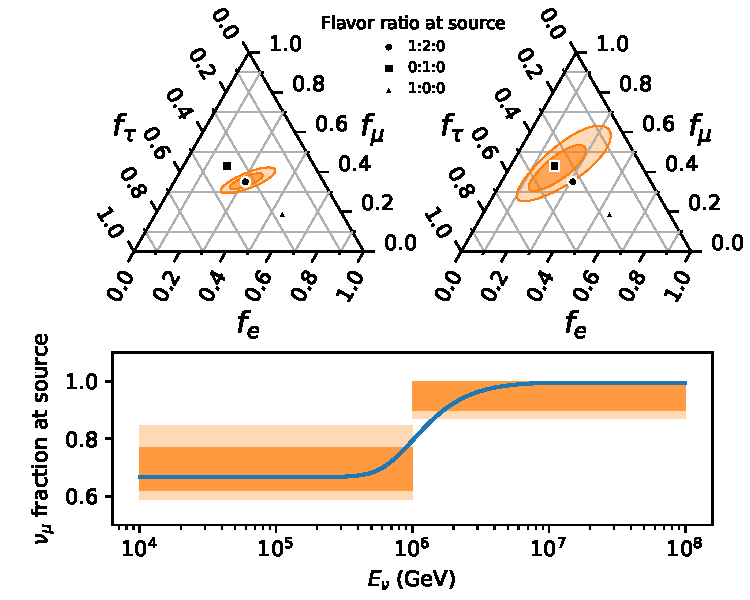
\includegraphics{./figures/gen2/MuonDamped.pdf}
    \caption[Sensitivity of IceCube-Gen2 to measure an energy dependent flavour composition of Astrophysical neutrino]{The bottom section displays the proportion of $\nu_{\mu}$ at the source based on energy, with the assumption that the muon critical energy is 2 PeV. The error bars represent the 68\% confidence level limitations on the $\nu_{\mu}$ fraction below and above 1 PeV, derived from the observed flavour composition of $\nu_{\mu}$ at Earth using IceCube-Gen2 and assuming standard oscillations. In the upper sections, the dark (light) shaded regions depict the corresponding 68\% (99\%) constraints, without making any assumptions about the mixing matrix.}
    \labfig{gen2_muondamped}
\end{figure}

The power of combining different event samples, extension of detector volume along with an isotropic module already shows a significant gain in sensitivity to measure flavour composition of astrophysical neutrinos. Furthermore, the optical component of IceCube Gen2 will also be sensitive to detect a changing flavour composition as a function of neutrino energy, that shall allow us to distinguish population of dominating sources across the spectrum. The study presented above can be further extended by adding the proposed radio component to the sample \sidecite{Coleman}. As described in Section~\ref{sec:gen2-detector}, due to the extended radio array IceCube-Gen2 shall be sensitive to measure EeV neutrinos as well \sidecite{Gen2_TDR}. \reffig{gen2_radioincluded_flavour} shows extension of sensitivity projection shown in \reffig{gen2_muondamped}, by adding flavour tagging at higher energies. It shows that at even higher energies, where the diffuse neutrino spectrum is dominated by cosmogenic neutrinos (see Section~\ref{sec:cosmogenic_nu}), the measure flavour ratio transitions back to the 1:2:0 scenario at the source \cite{Coleman}.  


\begin{figure*}[h!]
    \centering
        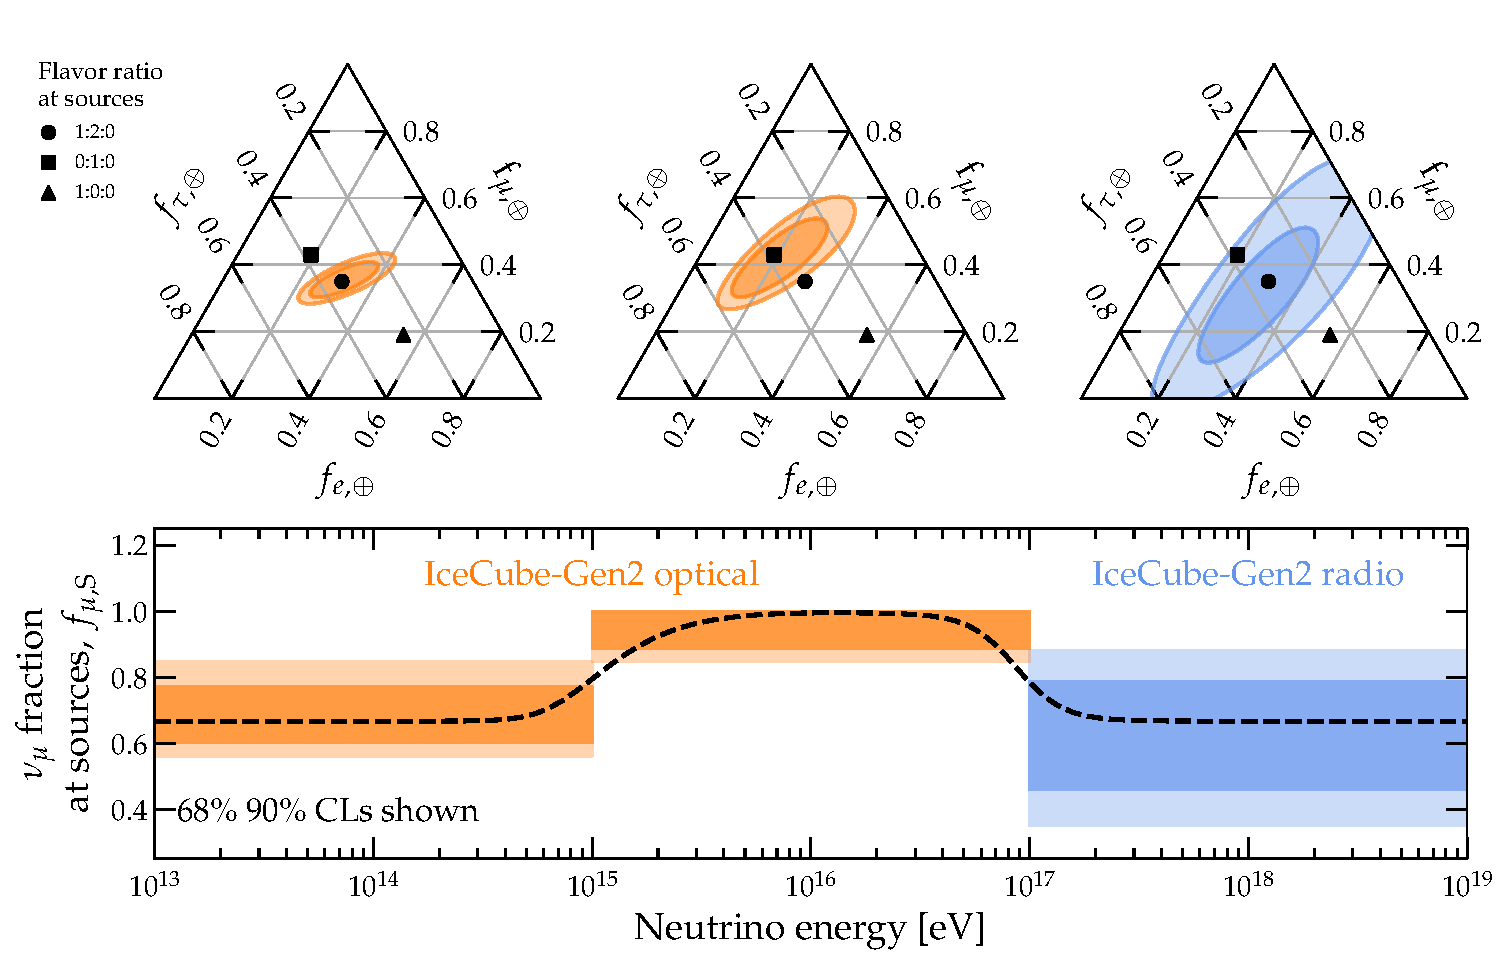
\includegraphics{./figures/gen2/energy_dependence_Gen2_TA-GZK.pdf}
        \caption[A combined sensitivity of IceCube-Gen2 to measure flavour composition of Astrophysical neutrino using both optical and radio components of the detector]{A combined sensitivity to measure evolution of the neutrino flavour composition with energy ranges from TeV to EeV range, using both optical and radio components of IceCube Gen2 Detector. Astrophysical neutrino sources are generally expected to be dominated by pion decay at the lowest energies, with a flavour composition of approximately (1:2:0). At intermediate energies, the sources transition to a muon-damped production regime, yielding a flavour ratio of roughly (0:1:0). Finally, at the highest energies, the composition reverts to the pion decay pattern, (1:1:1), as anticipated for cosmogenic neutrino production. The details for layout are similar to that shown in \reffig{gen2_muondamped}. The extended figure, taken from \cite{Coleman}.}
        \labfig{gen2_radioincluded_flavour}
    \end{figure*}

To conclude, IceCube-Gen2's increased volume will improve the detection rate of tau neutrinos, which are identifiable by their unique "double-bang" decay signature. This enhancement in tau neutrino identification, especially above 300 TeV, will provide critical insights into the flavour composition of astrophysical neutrinos, enabling stronger constraints on source physics and the potential to detect new physics beyond the Standard Model. Furthermore, the inclusion of a radio array may extend tau neutrino detection capabilities to even higher energies in the EeV range, offering unprecedented precision in exploring the universe's most extreme neutrino sources. The enhanced sensitivity of IceCube-Gen2, achieved through the combination of optical and radio detection methods, will close critical gaps in our understanding of the cosmic neutrino energy spectrum, extending the detection range up to three orders of magnitude higher than current capabilities. This leap in sensitivity will enable the discovery of ultra-high-energy neutrinos, paving the way for transformative progress in both high-energy physics and astrophysics. 